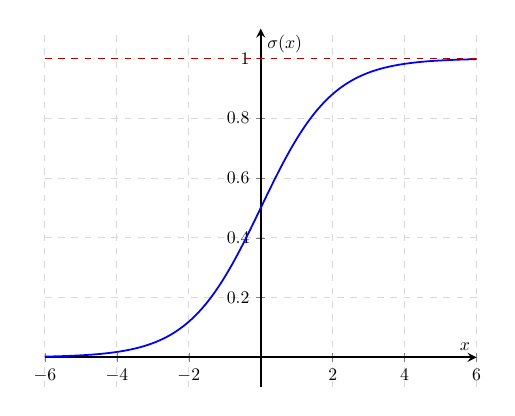
\begin{tikzpicture}[scale=0.8, every node/.style={scale=0.8}]
    \begin{axis}[
            axis lines = middle,
            xlabel = {$x$},
            ylabel = {$\sigma(x)$},
            xmin = -6, xmax = 6,
            ymin = -0.1, ymax = 1.1,
            domain = -6:6,
            samples = 100,
            smooth,
            thick,
            grid = major,
            grid style = {dashed, gray!30},
            legend pos = north west
        ]
        % Standard Logistic (Sigmoid) Function: f(x) = 1 / (1 + exp(-x))
        \addplot[color=blue] {1 / (1 + exp(-x))};

        % Asymptotic Boundaries y = 0 and y = 1
        \draw[dashed, red!70!black, thin] (axis cs:-6,1) -- (axis cs:6,1);

    \end{axis}
\end{tikzpicture}
